% Appendix Section
% This file contains supplementary material

\appendix
\onecolumn

\section{Implementation Details}
\label{app:details}

\subsection{Image Classification}

\paragraph{Pre-training.} We train DeiT models on ImageNet-1K following an improved training recipe. For DeiT-Base and DeiT-Small, we train for 300 epochs with a batch size of 4096, learning rate of $2 \times 10^{-4}$, weight decay of 0.3, and drop path rate of 0.1. For DeiT-Large, we train for 200 epochs with the same hyperparameters except drop path rate of 0.2. We use AdamW optimizer with $\beta_1 = 0.95$ and cosine learning rate schedule with 20 warmup epochs. We employ the same data augmentation pipeline during training as the original DeiT implementation.

\paragraph{Fine-tuning.} For fine-tuning at $224 \times 224$, we train for 20 epochs with learning rate $10^{-5}$, weight decay 0.1, and the same drop path rate as pre-training. For higher resolutions ($384 \times 384$ and $448 \times 448$), we fine-tune from the $224 \times 224$ checkpoint for 20 epochs with the same hyperparameters. We use full crop (crop ratio 1.0) during evaluation.

\paragraph{Spiral RoPE Configuration.} For all classification experiments, we use $K=16$ directions with base frequency scaling factor 1.5 (i.e., $\theta_{\text{base}} = 15000$). Spiral RoPE is combined with the original absolute positional embedding (APE).

\begin{table}[h]
    \caption{Pre-training hyperparameters for ImageNet-1K classification.}
    \label{tab:pretrain_hyperparams}
    \begin{center}
        \begin{tabular}{lcc}
            \toprule
            Hyperparameter & DeiT-Base and DeiT-Small & DeiT-Large \\
            \midrule
            Epochs & 300 & 200 \\
            Batch size & 4096 & 4096 \\
            Optimizer & AdamW & AdamW \\
            Learning rate & $2 \times 10^{-4}$ & $2 \times 10^{-4}$ \\
            Weight decay & 0.3 & 0.3 \\
            $\beta_1$, $\beta_2$ & 0.95, 0.999 & 0.95, 0.999 \\
            LR schedule & Cosine & Cosine \\
            Warmup epochs & 20 & 20 \\
            Drop path & 0.1 & 0.2 \\
            Label smoothing & 0.1 & 0.1 \\
            \midrule
            \multicolumn{3}{c}{\textit{Data Augmentation}} \\
            \midrule
            RandAugment & (9, 0.5) & (9, 0.5) \\
            Mixup $\alpha$ & 0.8 & 0.8 \\
            CutMix $\alpha$ & 1.0 & 1.0 \\
            Random erasing & 0.25 & 0.25 \\
            \midrule
            \multicolumn{3}{c}{\textit{Spiral RoPE Parameters}} \\
            \midrule
            Number of directions ($K$) & 16 & 16 \\
            Base frequency scale & 1.5 & 1.5 \\
            \bottomrule
        \end{tabular}
    \end{center}
\end{table}

\subsection{Semantic Segmentation}
We use UperNet as the segmentation framework with DeiT backbones initialized from ImageNet pre-trained weights at $224 \times 224$ resolution. Models are trained on ADE20K at $512 \times 512$ resolution for 160K iterations with a total batch size of 16 (8 GPUs $\times$ 2 samples per GPU). We use AdamW optimizer with learning rate $6 \times 10^{-5}$, weight decay 0.01, and polynomial learning rate decay with 1.5K warmup iterations. Weight decay is disabled for position embeddings, class tokens, normalization layers, and layer scale parameters. For Spiral RoPE models, we use the same $K=16$ and base frequency scale 1.5 as in classification.


\subsection{Image Generation}

We follow the training recipe of the original DiT implementation \cite{peeblesScalableDiffusionModels2023}. Specifically, we train DiT models on ImageNet $256 \times 256$ for class-conditional image generation. All models are trained for 400K steps with a global batch size of 256. We use the AdamW optimizer with a constant learning rate of $10^{-4}$ and no weight decay. We employ the EMA of model weights with decay 0.9999 for evaluation. For sampling, we use DDPM with 250 steps and classifier-free guidance scale of 1.0.
FID is computed on 50K generated samples using the ADM evaluation toolkit \cite{dhariwalDiffusionModelsBeat2021}.

\paragraph{Spiral RoPE Configuration.} 
For DiT experiments, we use $K=8$ for S, B, and L models, and $K=6$ for XL models. The base frequency scale is set to 1.5 for all models.

\begin{table}[h]
    \caption{DiT training hyperparameters.}
    \label{tab:dit_hyperparams}
    \begin{center}
        \begin{tabular}{lc}
            \toprule
            Hyperparameter & Value \\
            \midrule
            Training steps & 400K \\
            Global batch size & 256 \\
            Optimizer & AdamW \\
            Learning rate & $1 \times 10^{-4}$ \\
            Weight decay & 0.0 \\
            EMA decay & 0.9999 \\
            \midrule
            \multicolumn{2}{c}{\textit{Sampling}} \\
            \midrule
            Sampling steps & 250 \\
            CFG scale & 1.0 \\
            \midrule
            \multicolumn{2}{c}{\textit{Spiral RoPE Parameters}} \\
            \midrule
            $K$ (S/B/L) & 8 \\
            $K$ (XL) & 6 \\
            Base frequency scale & 1.5 \\
            \bottomrule
        \end{tabular}
    \end{center}
\end{table}

\section{Additional Generated Samples}
\label{app:samples}

We provide additional uncurated samples generated by our DiT-XL/2 model with Spiral RoPE, trained for 7 million steps on ImageNet $256 \times 256$. For each class, we show 40 randomly generated samples. All samples are generated using classifier-free guidance with scale 4.0.

\begin{figure}[h]
    \centering
    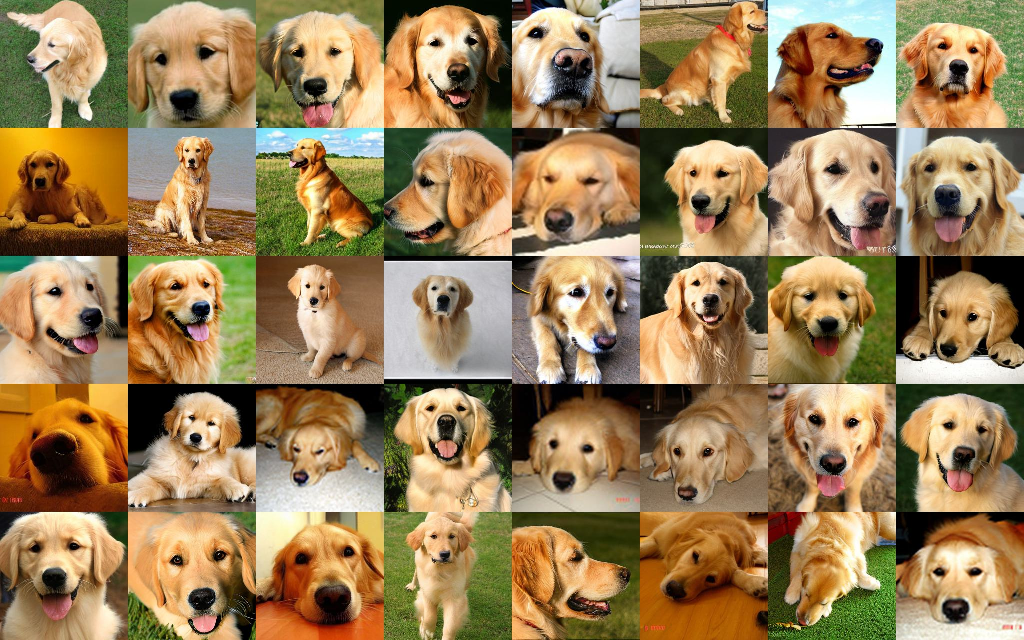
\includegraphics[width=0.9\textwidth]{plots/more_dit_examples/0207_golden_retriever_grid.pdf}
    \caption{Class 207: Golden Retriever}
\end{figure}

\begin{figure}[h]
    \centering
    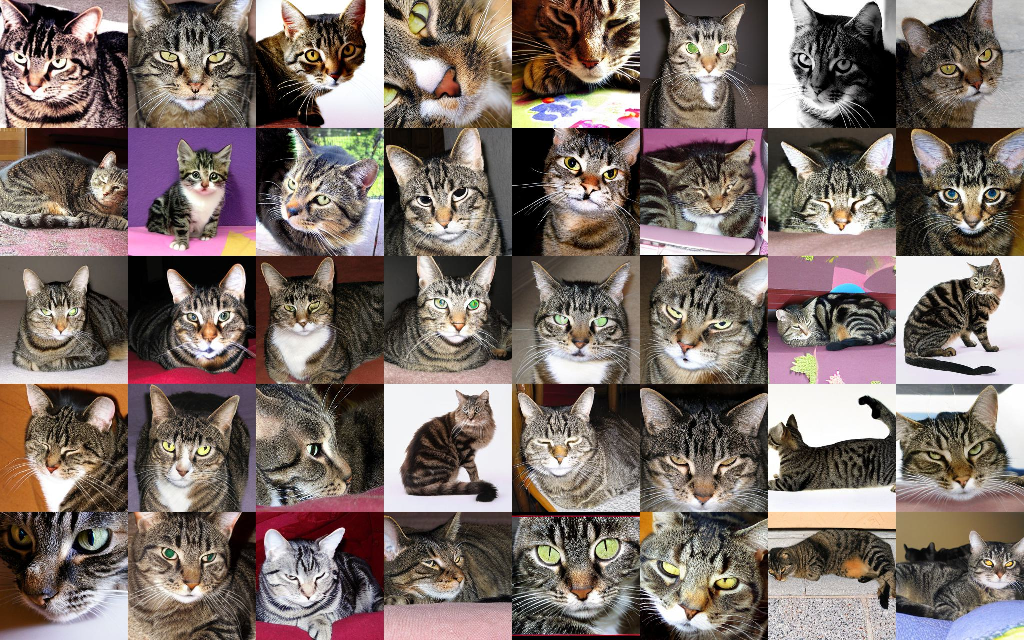
\includegraphics[width=0.9\textwidth]{plots/more_dit_examples/0281_tabby_cat_grid.pdf}
    \caption{Class 281: Tabby Cat}
\end{figure}

\begin{figure}[h]
    \centering
    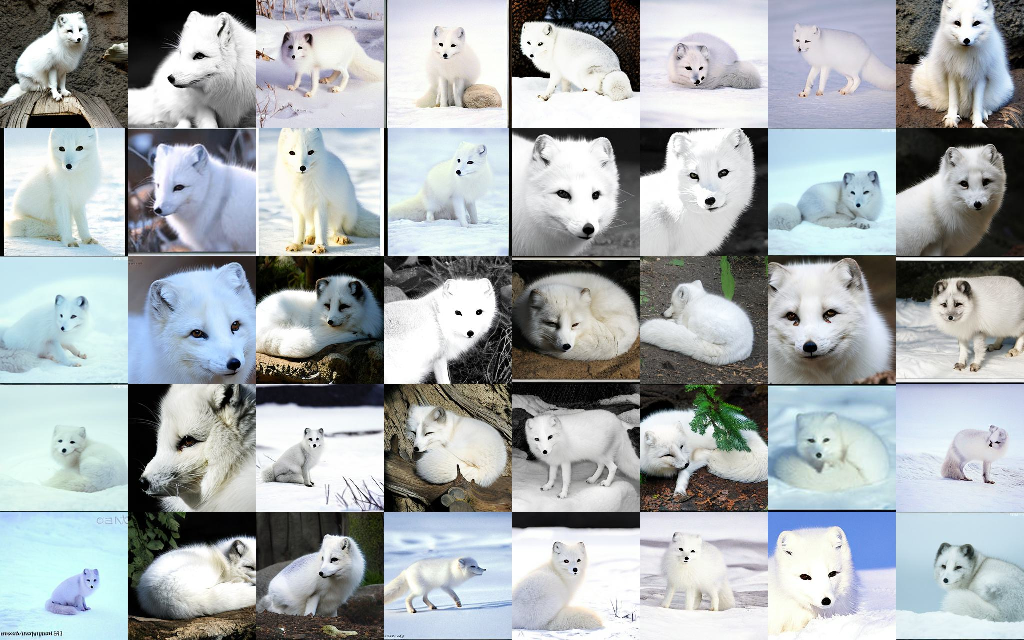
\includegraphics[width=0.9\textwidth]{plots/more_dit_examples/0279_arctic_fox_grid.pdf}
    \caption{Class 279: Arctic Fox}
\end{figure}

\begin{figure}[h]
    \centering
    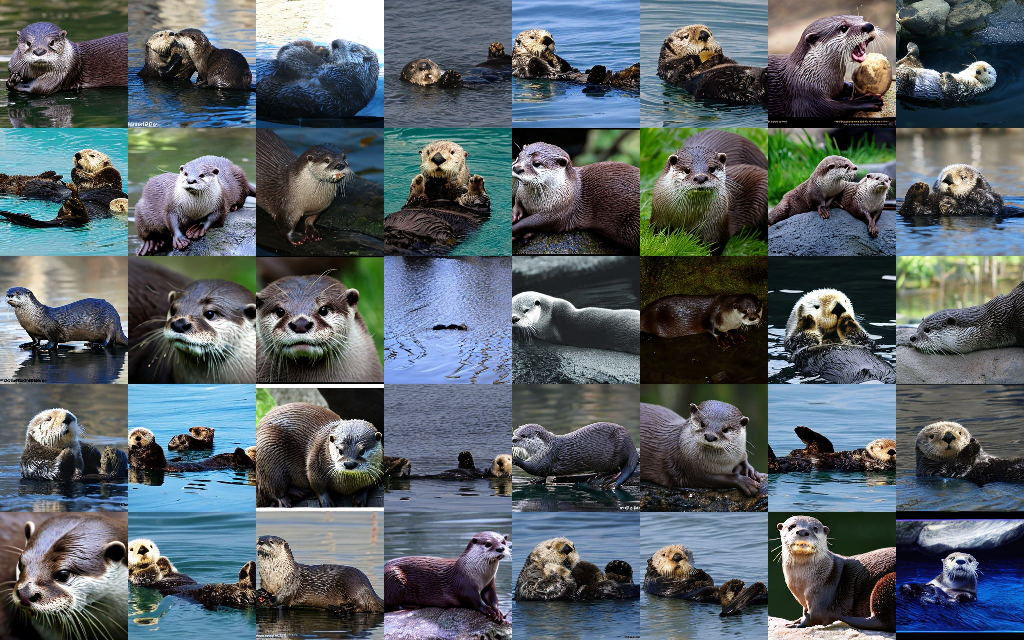
\includegraphics[width=0.9\textwidth]{plots/more_dit_examples/0360_otter_grid.pdf}
    \caption{Class 360: Otter}
\end{figure}

\begin{figure}[h]
    \centering
    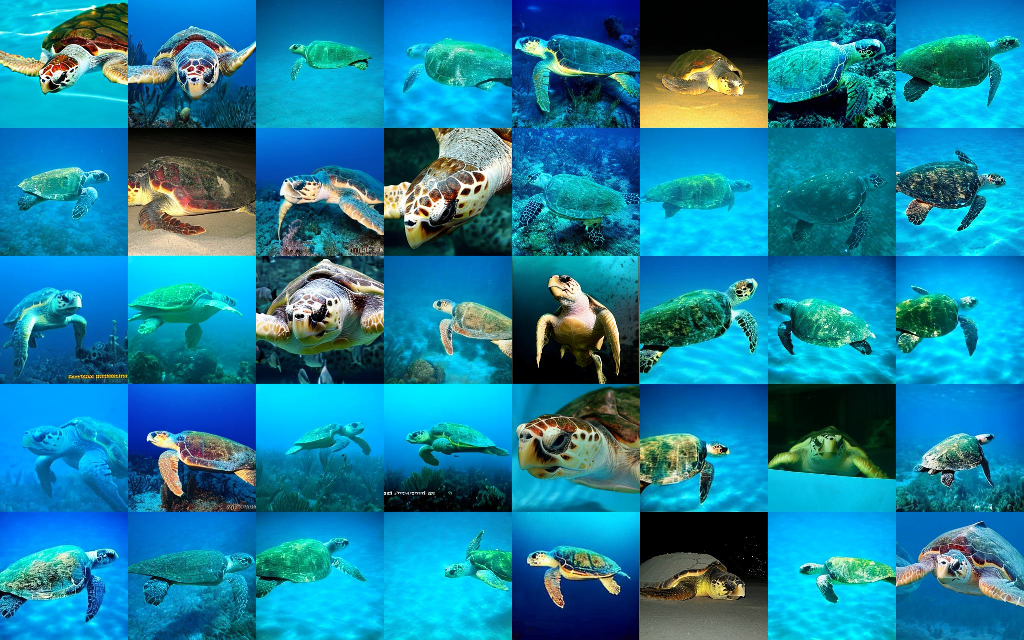
\includegraphics[width=0.9\textwidth]{plots/more_dit_examples/0033_loggerhead_turtle_grid.pdf}
    \caption{Class 33: Loggerhead Turtle}
\end{figure}

\begin{figure}[h]
    \centering
    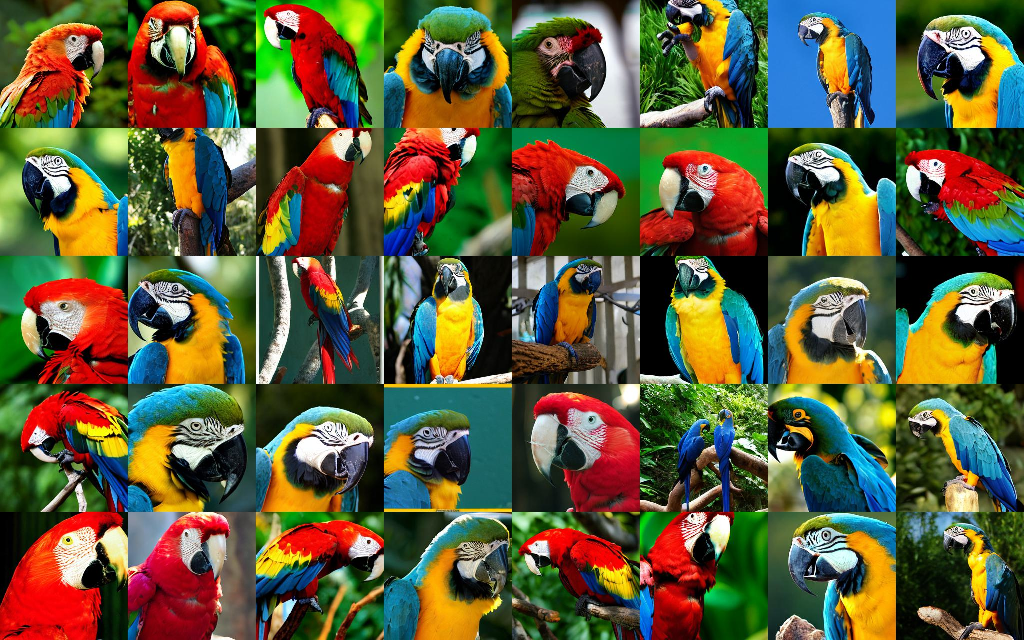
\includegraphics[width=0.9\textwidth]{plots/more_dit_examples/0088_macaw_grid.pdf}
    \caption{Class 88: Macaw}
\end{figure}

\begin{figure}[h]
    \centering
    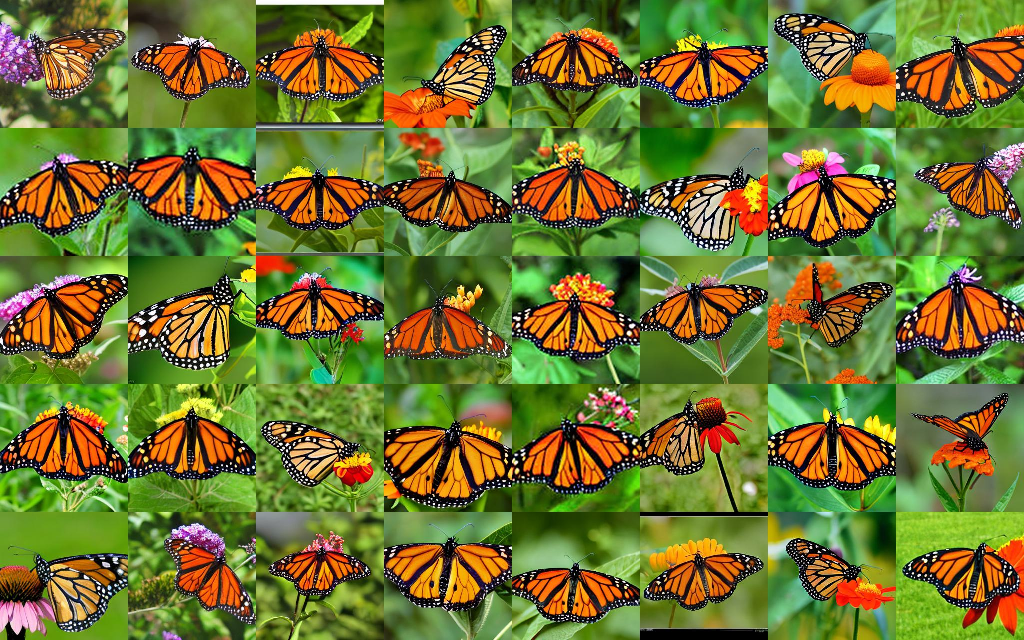
\includegraphics[width=0.9\textwidth]{plots/more_dit_examples/0323_monarch_butterfly_grid.pdf}
    \caption{Class 323: Monarch Butterfly}
\end{figure}

\begin{figure}[h]
    \centering
    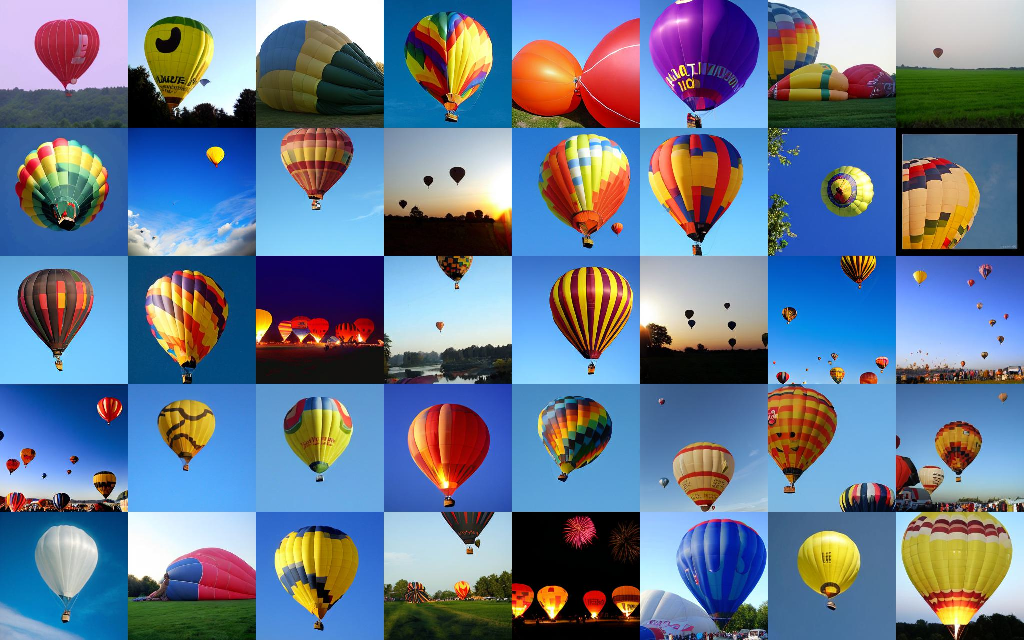
\includegraphics[width=0.9\textwidth]{plots/more_dit_examples/0417_balloon_grid.pdf}
    \caption{Class 417: Balloon}
\end{figure}

\begin{figure}[h]
    \centering
    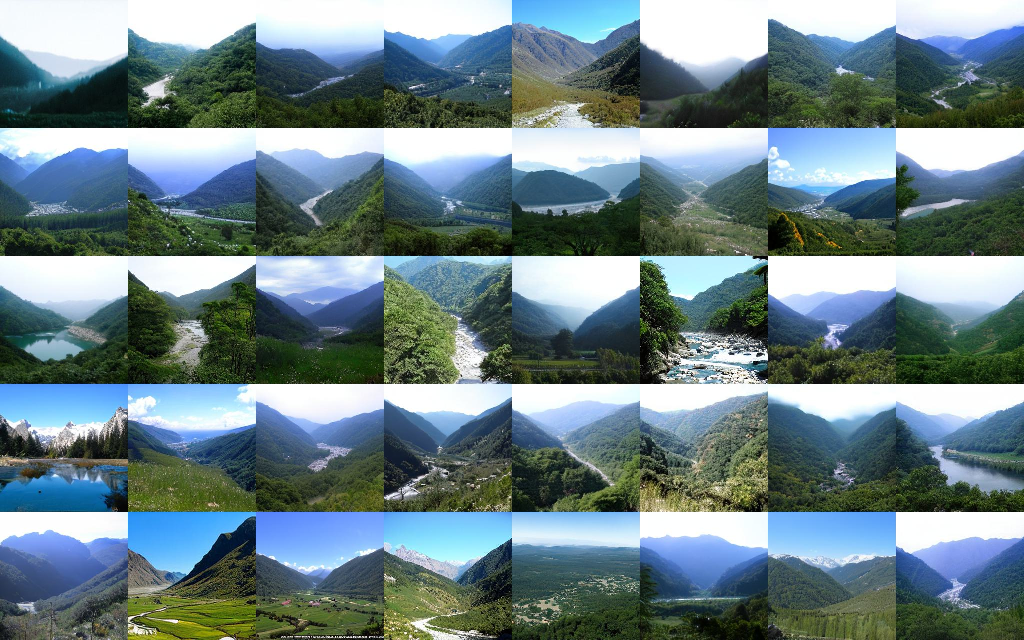
\includegraphics[width=0.9\textwidth]{plots/more_dit_examples/0979_valley_grid.pdf}
    \caption{Class 979: Valley}
\end{figure}

\begin{figure}[h]
    \centering
    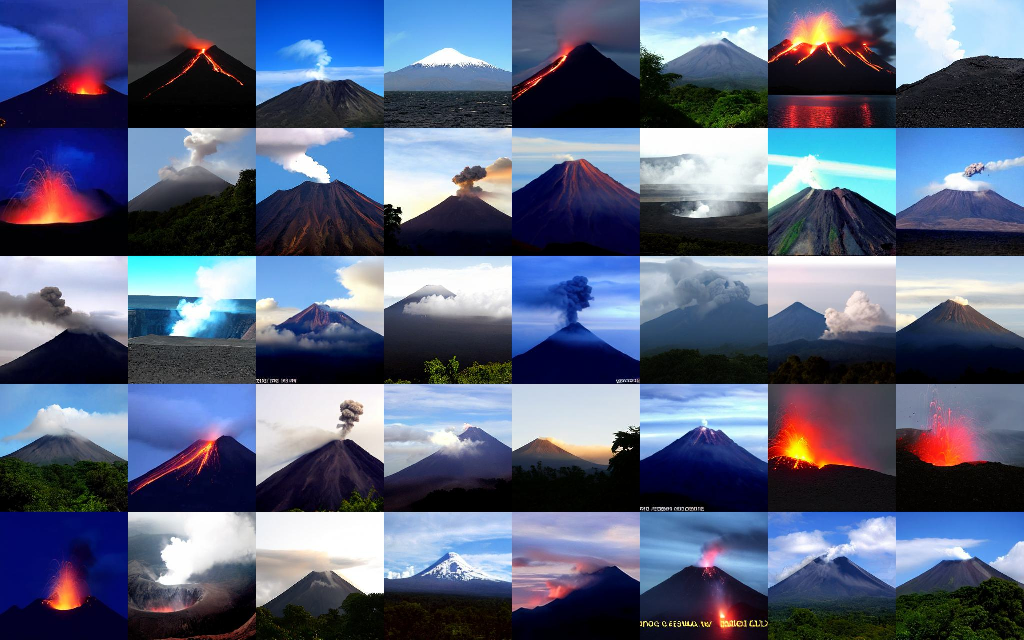
\includegraphics[width=0.9\textwidth]{plots/more_dit_examples/0980_volcano_grid.pdf}
    \caption{Class 980: Volcano}
\end{figure}
